\chapter{ParaCoND: Paralog-specific Gene Copy Number Discovery}
In this chapter, each step that we followed in our method will be explained in detail.
\section{Structural Variation Discovery with HTS Data}
Structural variations are believed to be highly associated with diseases \cite{fanciulli2007fcgr3b,fellermann2006chromosome,aitman2006copy,gonzalez2005influence}. Therefore their discovery will be of critical importance in reducing the genetic disease susceptibility. Despite their significance in understanding disease susceptibility, there is no algorithm yet to find all types and sizes of structural variations at once. Before high-throughput sequencing technologies, microarrays were mainly used in structural variation discovery especially for copy number variation \cite{alkan2011genome}. As reviewed by Alkan et al., microarrays are not good at discovering balanced rearrangements and also are not able to locate the copy number variations \cite{alkan2011genome}. 

Although some are originally designed for old sequencing technologies, high-throughput sequencing platforms have brought novel methods for structural variation discovery. 
\subsection{Read Pair}
Paired-end sequencing is a sequencing method where reads are generated from both sides of a DNA fragment whose distance is known. The distance information will be used later by the aligner while aligning the paired-end reads to the reference genome. Read pair method utilizes the distance information between paired-end reads \cite{tuzun2005fine}. As shown in the Figure \ref{readpair}, paired-end reads that align too distant from each other indicates a deletion, those align too close to each other indicates an insertion.

\begin{figure}[ht]
    \centering
    \caption{Structural variation discovery with read pair}
    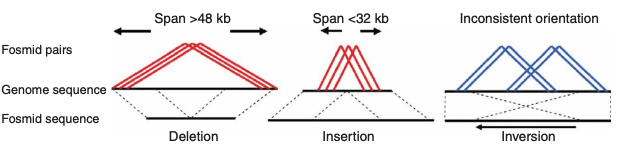
\includegraphics[scale=0.4]{images/readpair.png}
    \caption*{Paired-end reads that are mapped too distant from each other indicates deletion, too close to each other indicates insertion and ahead of what should be behind indicates inversion (adapted from \cite{tuzun2005fine})}
    \label{readpair}
\end{figure}

Structural variation discovery tools based on read-pair can be categorized as follows:
\begin{itemize}
    \item Unique Mapping: PEMer \cite{korbel2009pemer}, BreakDancer \cite{chen2009breakdancer}, GenomeSTRIP \cite{handsaker2015large}, 
    \item Multiple Mapping: VariationHunter \cite{hormozdiari2009combinatorial}, CommonLAW \cite{hormozdiari2011simultaneous}, MoDIL \cite{lee2009modil}, MoGUL \cite{lee2010mogul}, HYDRA \cite{quinlan2010genome}
\end{itemize}
\subsection{Read Depth}
Read depth is a simple method to detect duplications and deletions. Based on the assumption that regions are randomly sequenced, for reads that are mapped to the reference genome, the depth of duplicated regions will be higher and the depth of deleted regions will be lower than average \cite{bailey2002recent} as shown in Figure \ref{readdepth}. Multiple read-mapping is an important aspect of read depth to work effectively. Otherwise the difference of depth between duplicated regions and deleted regions will be insignificant. However known sequencing bias against GC-rich and GC-poor regions \cite{smith2008rapid} should be handled carefully.

\begin{figure}[ht]
    \centering
    \caption{Structural variation discovery with read depth}
    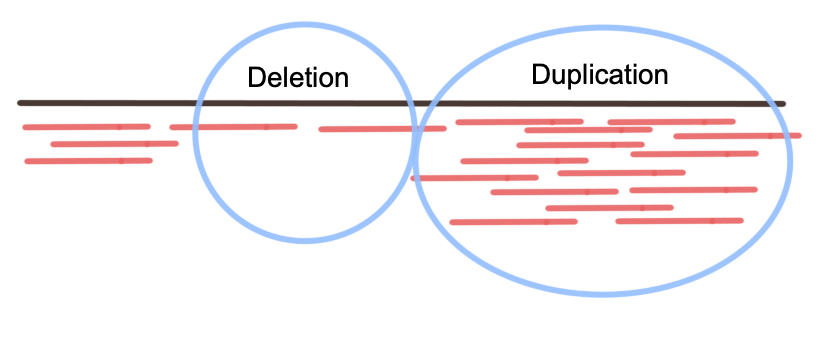
\includegraphics[scale=0.7]{images/readdepth.png}
    \caption*{The depth of regions that are duplicated will be higher and the depth of regions that are deleted will be lower than expected depth}
    \label{readdepth}
\end{figure}

Structural variation discovery tools based on read depth can be categorized as follows:
\begin{itemize}
    \item Unique Mapping: CNVnator \cite{abyzov2011cnvnator}, Event-Wise Testing \cite{yoon2009sensitive}
    \item Multiple Mapping: Whole Genome Shotgun Sequence \cite{bailey2002recent}, mrCaNaVar \cite{alkan2009personalized}
\end{itemize}

\subsection{Split Read}
Originally designed for longer reads (Sanger sequence etc.), split read based methods were capable of structural variation discovery at one base pair resolution by trying to map the reads by splitting. Similar to read pair, the location of split reads will tell the class of structural variation. For instance, the distance between split reads shows an insertion or first split coming after second split indicates an inversion.

Structural variation discovery methods based on split read can be categorized as follows:
\begin{itemize}
    \item Unique Mapping: Pindel \cite{ye2009pindel}, SRiC \cite{zhang2011identification}
    \item Multiple Mapping: Splitread \cite{karakoc2012detection}
\end{itemize}

\subsection{Sequence Assembly} 
Although it is in its early stages, sequence assembly methods are, in theory, powerful and requires less computational power. Assuming the whole genome is assembled without using the reference genome (\textit{de novo} assembly), we can easily detect structural variation by comparing the individual's genome with the reference genome. NovelSeq \cite{hajirasouliha2010detection}, PopIns \cite{kehr2015popins} can be examples of this type.

\subsection{Hybrid Methods}
There are also some methods using two or more of these techniques in order to increase their accuracy. Examples of these type of methods can be DELLY \cite{rausch2012delly} in which read pair and split read were used, LUMPY \cite{layer2014lumpy} in which read pair, read depth and split read were used, TARDIS \cite{soylev2017toolkit} in which read pair, read depth and split read were used.

\section{Dataset}
We have the data showing the genome-wide segmental duplications (SD). The data is coming from Segmental Duplication Database of UW Genome Sciences Human Paralogy Laboratory \cite{she2004shotgun, bailey2002recent}. The data consist of 51,599 SD pairs with their exact locations. Furthermore, we have global alignments of SD pairs in files generated using a sequence alignment tool called ClustalW \cite{thompson1994clustal}.

\section{Data Preprocessing}
\begin{sidewaysfigure}[ht]
    \centering
    \caption{Workflow figure of ParaCoND}
    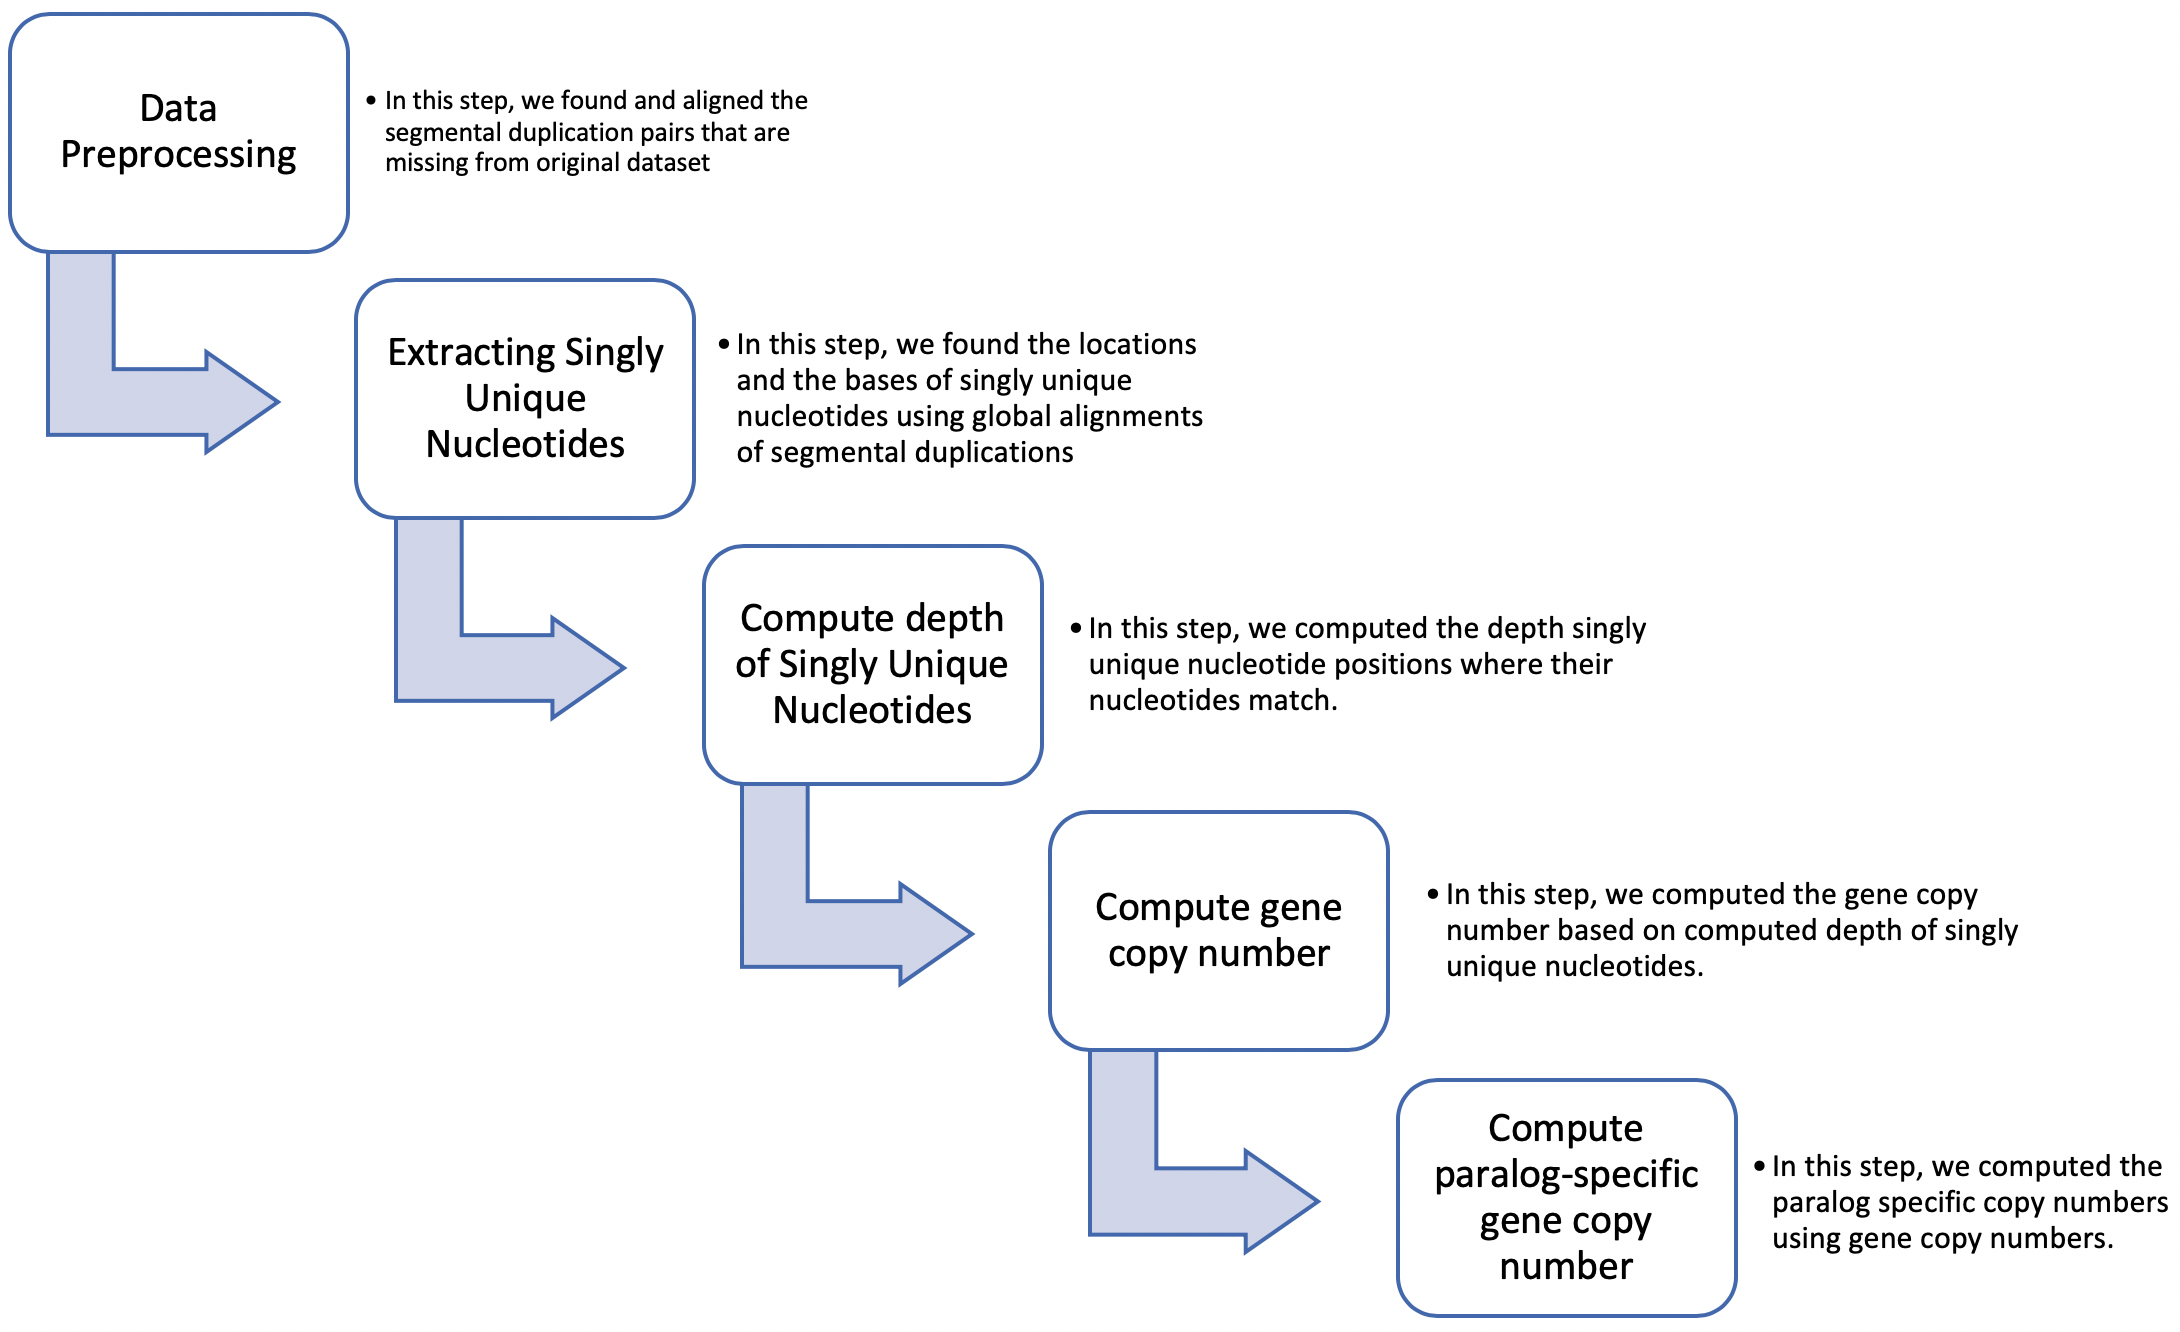
\includegraphics[scale=0.55]{images/workflow.png}
    \label{workflow}
\end{sidewaysfigure}

Since entries in our data show the duplications in pairs, we had to turn these pairs into a multiple sequence alignment in order to locate singly unique nucleotide positions. However, our data lack some pairs. For example, we have SD pairs of A-B and B-C, therefore A-C should also be in our data whereas there is not in some cases. Using the Algorithm \ref{missingPairs}, we have identified 21,023 new SD pairs using existing pairs and have them aligned.

\begin{algorithm}
\caption{An algorithm to find missing SD pairs}
\label{missingPairs}
\begin{algorithmic}[1]
\Procedure{Find\_Missing\_Pairs}{}
\State $\textit{M} \gets \text{map of }\textit{Segmental Duplications}\text{ as read from data}$
\For{$\text{each key-value pair in }\textit{M}$}
\State {$\text{Let } \textit{temp\_set} \text{ be an empty set} $}
\For{$\text{values in M{[key]}}$}
\State $\textit{temp\_set} \gets \textit{temp\_set} \cup \text{M{[value]}}$
\State $\text{clear M{[value]}}$
\EndFor
\While{true}
\State $\textit{flag} \gets \text{true}$
\For{$\text{each key-value pair in }\textit{M}$}
\State $\textit{Find intersection of }\textit{temp\_set}\text{ and }\textit{value}$
\If{$\text{intersection is not empty}$}
\State $\textit{temp\_set} \gets \textit{temp\_set} \cup \text{M{[value]}}$
\State $\textit{flag} \gets \text{false}$
\EndIf
\EndFor
\If{$ \textit{flag} \text{ is true} $}
\State $\textbf{break}$
\EndIf
\EndWhile
\EndFor
\EndProcedure
\end{algorithmic}
\end{algorithm}

\section{Singly Unique Nucleotides} \label{section:sun}
Structural variation discovery has always been problematic since they tend to overlap with segmental duplications \cite{sudmant2010diversity}. Researchers that were unable to discriminate slight differences in these regions which prevents copy number variation from being accurately predicted have excluded these highly active regions from their studies. They have instead focused on unique regions of the genome.

In nearly identical regions, nucleotide difference information can be useful in discriminating segmental duplications from each other. Singly unique nucleotide (SUN) is a nucleotide difference between segmental duplications as shown red in figure \ref{singlyUniqueNucleotide}. A nucleotide difference is called a SUN if and only if they reside in only one paralog. Otherwise, as shown blue in the figure, they are called  paralogous sequence variant (PSV). 
\begin{figure}[ht]
    \centering
    \caption{Singly unique nucleotides and paralog specific variants}
    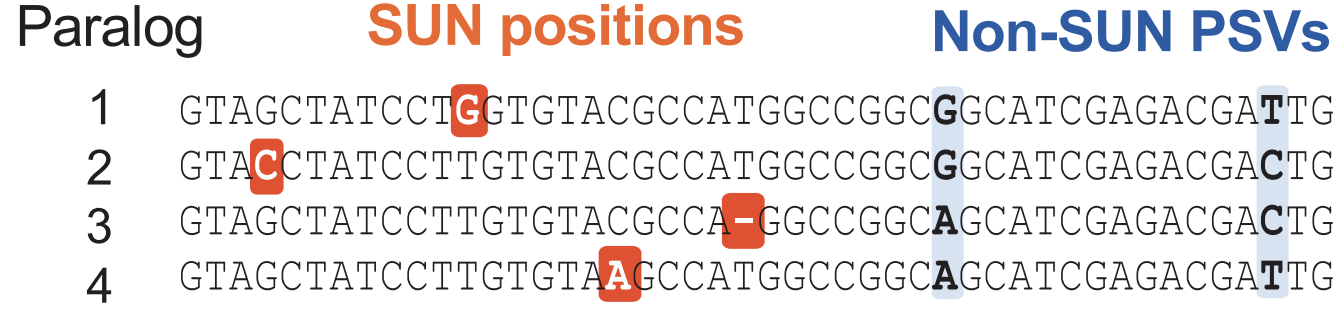
\includegraphics[scale=0.4]{images/singlyUniqueNucleotide.png}
    \caption*{Singly unique nucleotides are single nucleotide differences among segmental duplications. If there are more than one paralog that contains a nucleotide difference, it will be called a paralog specific variant (adopted from \cite{sudmant2010diversity})}
    \label{singlyUniqueNucleotide}
\end{figure}

\subsection{Extracting Singly Unique Nucleotides}
In order for paralogous sequences to be accurately identified, we need a database of positions and letters of all SUNs that reside in a segmental duplication. Instead of aligning paralogs using a multiple sequence alignment tool, which requires quite some time and computational power, it could be done using pairwise alignments of paralogs which we have in our hand (Figure \ref{alignmentFile}). Let $A$, $B$ and $C$ are three paralogs and  $S_{ab}$ denotes the singly unique nucleotides of $A$ relative to $B$. The singly unique nucleotides of A will be $S_{ab} \cap S_{ac}$. The same equation is valid for other paralogs respectively. Therefore, we could figure out all SUN positions as $(S_{ab} \cap S_{ac}) \cup (S_{ba} \cap S_{bc}) \cup (S_{ca} \cap S_{cb})$.

\begin{figure}[ht]
    \centering
    \caption{A sample screenshot from an alignment file}
    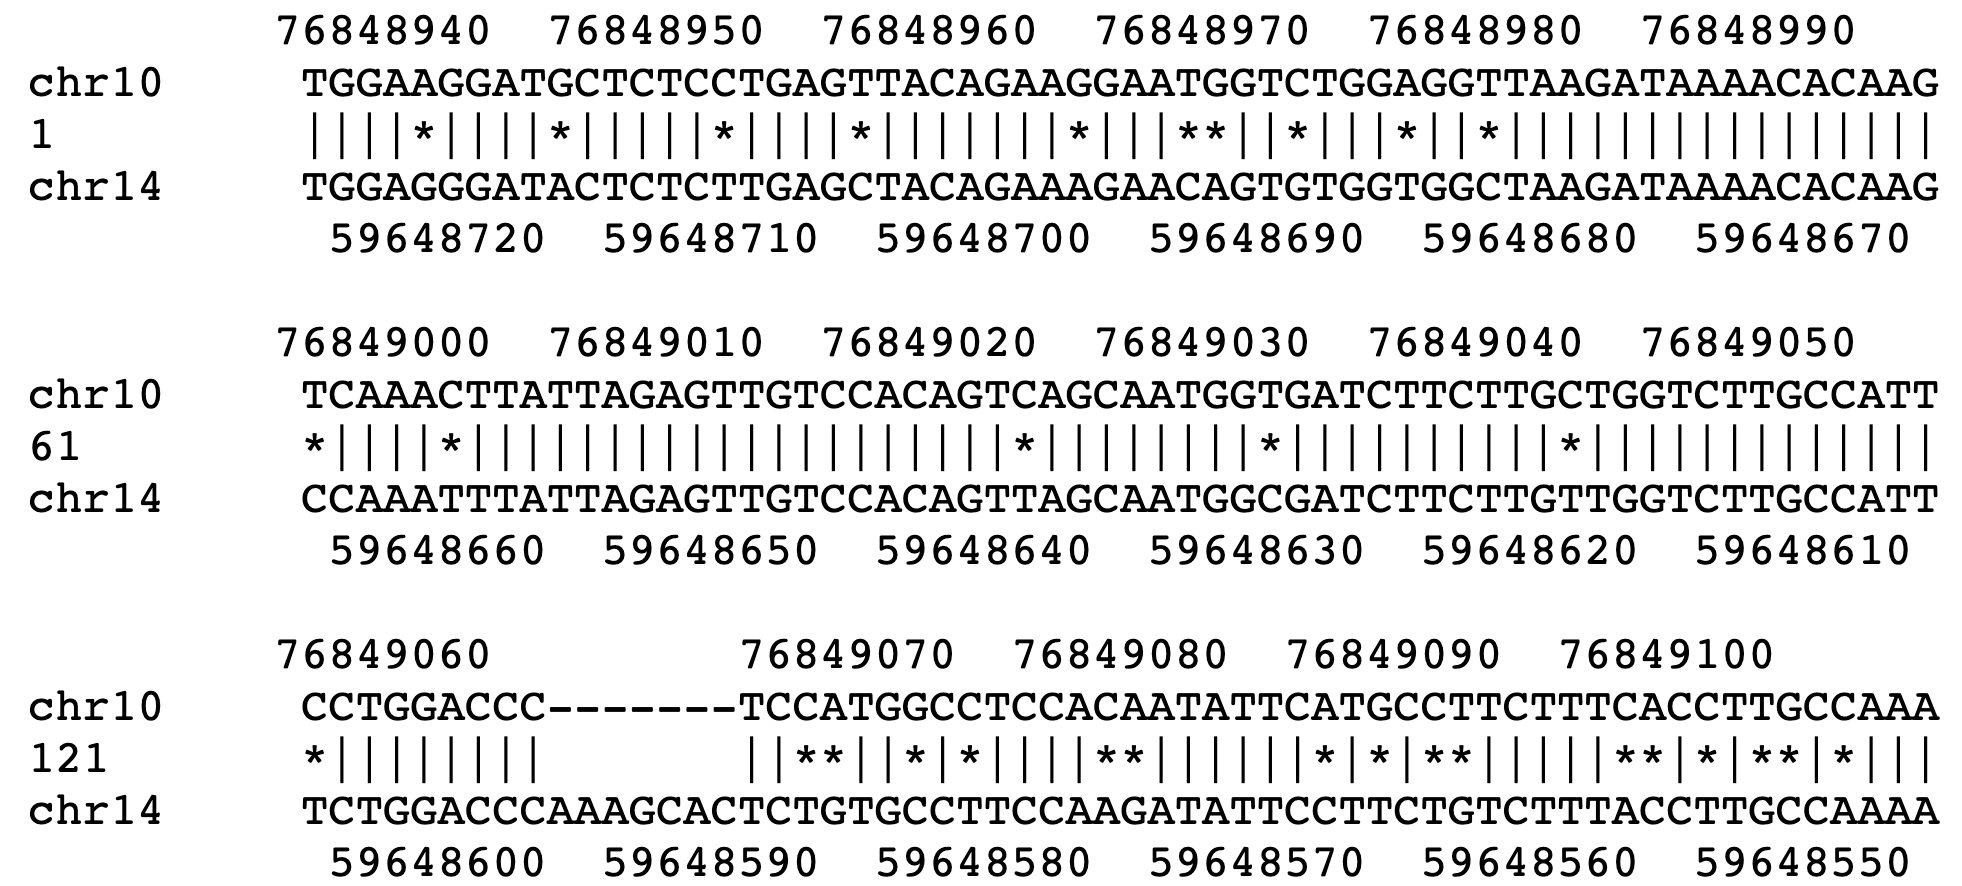
\includegraphics[scale=0.4]{images/alignmentFile.png}
    \label{alignmentFile}
\end{figure}

Algorithm \ref{getRelativeSun} uses an alignment file to find the pairwise SUN positions and letters. As shown in figure \ref{alignmentFile}, an alignment file contains the DNA sequences of two segments and an alignment results between them. The symbols $*$, $|$ and space denote a match, a mismatch and an indel respectively. It is important to state that, if there is a deletion in one sequence, every nucleotide position opposite of the deletion will be counted as a SUN. On the other hand, the deletion will be counted as one SUN. Another thing to pay attention is the strand of the sequences. Segmental duplications can be found in opposite strand of the DNA. In that case, the nucleotide in the alignment file will be replaced by its complement before getting saved to SUN database.

In algorithm \ref{allSun}, we use algorithm \ref{getRelativeSun} to create a SUN database of segmental duplications by intersecting relative SUN sets. First we find SUNs of A relative to B and SUNs of B relative to A. And then, if A or B come out for the first time, we save the relative SUNs directly to the \textit{sun\_map} since there is no set of SUNs yet to intersect. On the other hand, if A or B is found in \textit{sun\_map}, we intersect the old set of SUNs with the relative SUNs. We store the database in a map where its keys are segmental duplications and its values are SUN locations and letters.

As a result, we have found 15,352,106 unique SUN locations together with their bases on a positive strand of the DNA. 

\begin{algorithm}
\caption{An algorithm to find pairwise SUN locations and letters}
\label{getRelativeSun}
\begin{algorithmic}[1]
\Procedure{Get\_Relative\_SUN}{alignment\_file\_path, strand}
\State $\text{Open alignment file}$
\If{file is open}
\State $\text{Let } S_{ab} \text{ and } S_{ba} \text{ empty sets}$
\While{getline(file) $\neq$ EOF}
\State{seq1 $\gets$ getline(file)}
\State{aligment $\gets$ getline(file)}
\State{seq2 $\gets$ getline(file)}
\For{$ i\gets0 \text{ to size of } \textit{alignment}$}
\If{$\textit{strand} \text{ is } -1$}
\State{seq2[i] $\gets$ \textit{GET\_OPPOSITE\_PAIR}(seq2[i]) /* It} 
\State{returns the complement of the input nucleotide, for example} 
\State{if input is A, T is returned etc.*/}
\EndIf
\If{alignment[i] is `*'}
\State{$S_{ab} \gets S_{ab} \cup seq1[i]$}
\State{$S_{ba} \gets S_{ba} \cup seq2[i]$}
\EndIf
\If{alignment[i] is ` '}
\If{seq1[i] is `-'}
\State{$S_{ba} \gets S_{ba} \cup seq2[i]$}
\EndIf
\If{seq2[i] is `-'}
\State{$S_{ab} \gets S_{ab} \cup seq1[i]$}
\EndIf
\EndIf
\EndFor
\EndWhile
\EndIf
\EndProcedure
\end{algorithmic}
\end{algorithm}


\begin{algorithm}
\caption{An algorithm to find all SUN locations and letters}
\label{allSun}
\begin{algorithmic}[1]
\Procedure{Get\_All\_SUN}{duplication\_file\_path}
\State $\text{Open duplication file}$
\If{file is open}
\State {Let \textit{sun\_map} an empty map showing segmental duplication and }
\State {its SUN locations as key-value pair}
\For{each entry in duplication file}
\State{Let A, B segmental duplications as parsed from duplication file}
\State{$\text{alignment\_file\_path} \gets \text{parsed from duplication file}$}
\State{$\text{strand} \gets \text{parsed from duplication file}$}
\State{$S_{ab}\text{, } S_{ba} \gets \textit{GET\_RELATIVE\_SUN}(\text{alignment\_file\_path, strand})$}
\If{A exists in sun\_map}
\State{$\text{sun\_map[A]} \gets \text{sun\_map[A]} \cap S_{ab}$}
\Else
\State{$\text{sun\_map[A]} \gets S_{ab}$}
\EndIf
\If{B exists in sun\_map}
\State{$\text{sun\_map[B]} \gets \text{sun\_map[B]} \cap S_{ba}$}
\Else
\State{$\text{sun\_map[B]} \gets S_{ba}$}
\EndIf
\EndFor
\EndIf
\EndProcedure
\end{algorithmic}
\end{algorithm}
\section{Depth of Singly Unique Nucleotides}
The depth or coverage, a term that entered the literature thanks to the next generation sequencing, is defined as the number of `reads' that include a particular nucleotide. In next generation sequencing, the DNA is separated into little and overlapping portions, called `reads', to be assembled later. When the reads are aligned with respect to their mapping locations, nucleotides are sequenced in varying numbers as shown in figure \ref{depthOfCoverage}. Therefore the number the nucleotide gets sequenced is called the depth of that position.

As explained in Section \ref{section:sun}, we have created a SUN database showing all the SUN locations. In Algorithm \ref{findDepth}, we basically compute the depth of SUN locations if base in `read' matches with the base of SUN. In order to use this function, we need a BAM file as a parameter. BAM \cite{li2009sequence} is a file type for storing sequence alignment data in binary format. For each alignment it contains read name, read sequence, read quality, alignment information, and custom tags. We used HTSLib \cite{htslib}, a C library for reading/writing high-throughput sequencing data, to efficiently read a BAM file.
\begin{figure}[ht]
    \centering
    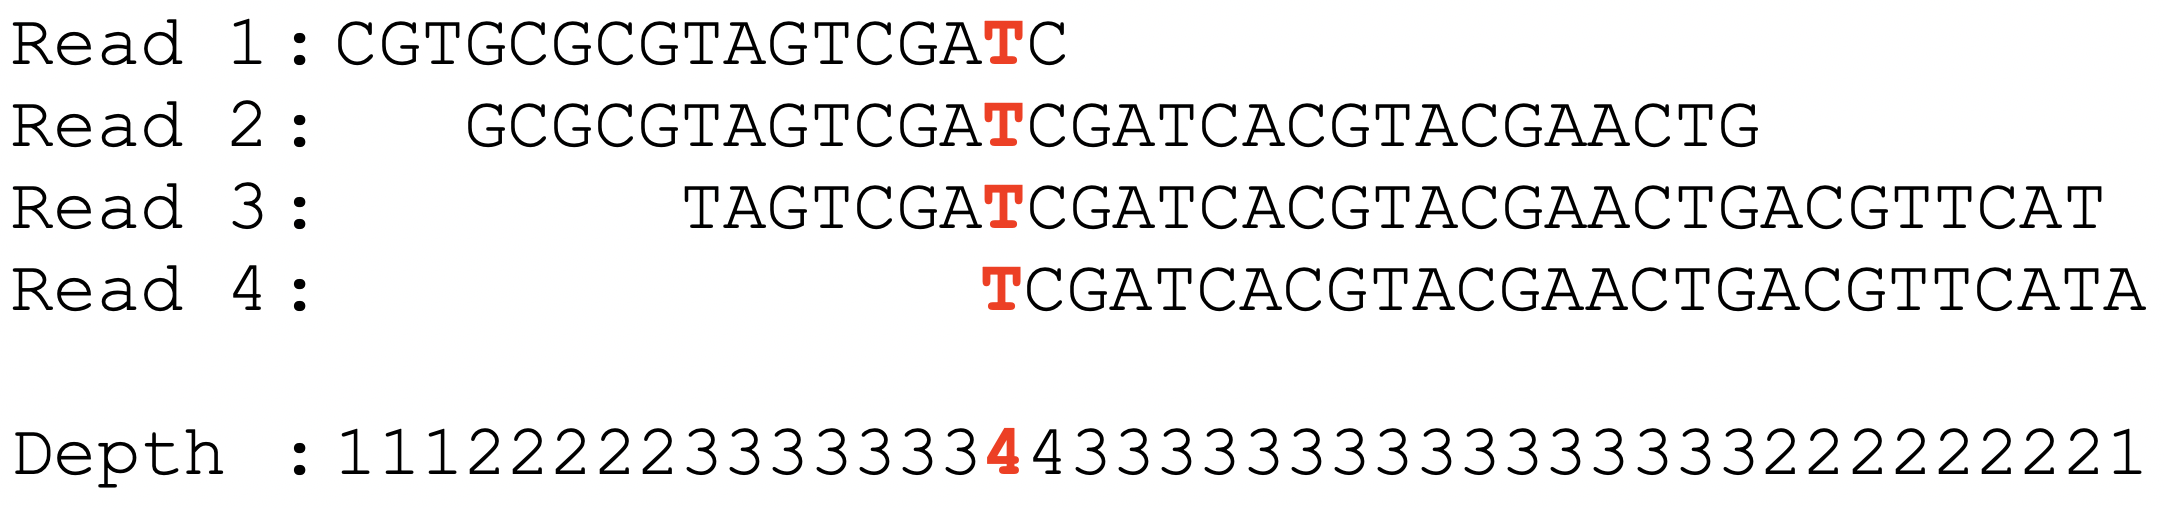
\includegraphics[scale=0.4]{images/depthofcoverage.png}
    \caption{Sequencing coverage (depth)}
    \label{depthOfCoverage}
\end{figure}
\begin{algorithm}
\caption{An algorithm to find depth of SUN locations}
\label{findDepth}
\begin{algorithmic}[1]
\Procedure{Find\_Depth}{bam\_file, sun\_set}
\State $\text{Open bam\_file}$
\If{file is open}
\For{every read in bam\_file}
\State $\text{chr} \gets \text{parsed from bam\_file}$
\State $\text{pos} \gets \text{parsed from bam\_file}$
\State $\text{len} \gets \text{parsed from bam\_file}$
\State $\text{seq[len]} \gets \textit{CONVERT\_ID\_TO\_NUCLEOTIDE}$ // In a bam file, 
\State each base is encoded in 4 bits: 0001: A, 0010: C, 0100: G, 
\State 1000: T, 1111: N. This procedure converts the binary-coded 
\State nucleotide to its letter representation.
\For{each SUN falling into the `reads' range}
\If{seq[SUN\_index] is equal to SUN nucleotide}
\State Increment depth of SUN by 1
\Else
\State Remove from sun\_set
\EndIf
\EndFor
\EndFor
\EndIf
\EndProcedure
\end{algorithmic}
\end{algorithm}

\subsection{GC Correction}
The next generation sequencing platforms are known to be biased against regions that are rich or poor in terms of GC content \cite{smith2008rapid}. This has been a known issue of NGS platforms that lead to uneven or even no coverage of reads across the genome. Unless it was handled carefully, structural variation discovery methods that rely on coverage data would not be applicable. Fortunately, there are statistical methods out there to fix the uneven distribution of reads. We used multiplicative version of locally weighted scatter plot smooth \cite{cleveland1991computational}, LOWESS or LOESS in short, to smooth our GC content vs read depth curve. The method starts with computing the average read depth of non-overlapping sequence windows of size 1 kilobase. Then the sequence windows are binned according to their GC percentage. There is 0.1\% difference between two consecutive bins. And again we compute the average read depth for each bin.
\begin{figure}[ht]
    \centering
    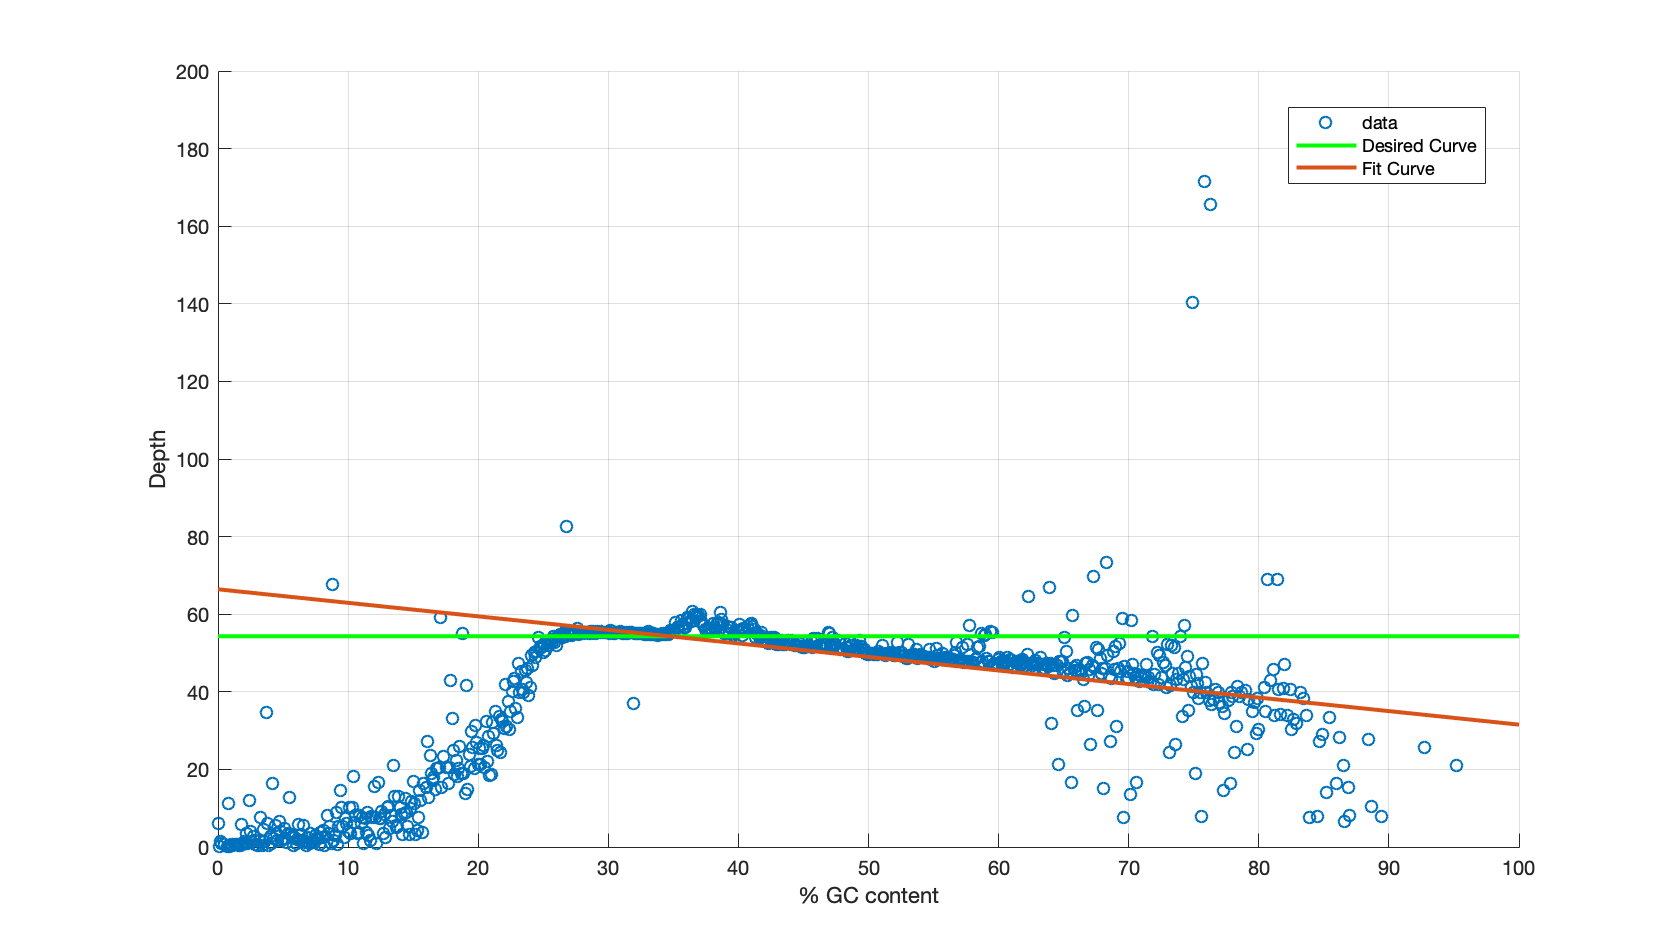
\includegraphics[scale=0.25]{images/gcCorrection.png}
    \caption{The average depth of 1 kb windows with respect to their GC content for NA12878}
    \label{gcCorrection}
\end{figure}
The figure \ref{gcCorrection} shows how the average read depth is impacted by GC content. The average read depth are getting lower with increasing GC content. We need to adjust the red line so that it comes closer to the green line. In multiplicative version of LOESS method, we define a correction factor, $k_{gc}$, which is equal to $$k_{gc} = \frac{\mu_{total}}{\mu_{gc}}$$ where $\mu_{total}$ is the average read depth of all sequence windows (i.e. green line) and $\mu_{gc}$ is the fit curve smoothed by LOESS (i.e. red line). Having computed $k_{gc}$ for all GC percentages and known the old value for read depth $d$,  new value for read depth, $d^\prime$, is calculated as; $$d^\prime = d*k_{gc}$$.

\section{Gene Copy Number}
Copy number variation is a structural variation that changes the amount of DNA. The simple yet powerful method for finding absolute copy number of a region is read depth. However, without multiple read mapping, applying read depth will give poor results. What we compute here is a copy number that will be useful later while computing the paralog specific copy number.

\begin{algorithm}
\caption{An algorithm to find gene copy number}
\label{findGeneCopyNumber}
\begin{algorithmic}[1]
\Procedure{Find\_Gene\_Copy\_Number}{gene\_file\_path, sun\_set}
\State Let \textit{Genes} be a vector of genes as read from gene\_file\_path
\For{each \textit{gene} in \textit{Genes}}
\State Let \textit{temp} be empty vector
\For{each SUN in sun\_set}
\If{SUN is in \textit{gene}}
\State Add read depth of SUN to \textit{temp}
\EndIf
\EndFor
\If{\textit{temp} is not empty}
\State {Compute mean and median of \textit{temp}}
\EndIf
\EndFor
\EndProcedure
\end{algorithmic}
\end{algorithm}

In algorithm \ref{findGeneCopyNumber}, we try to find average gene copy numbers using only the depth information of SUNs residing in that gene. The procedure takes two parameters. One is the \textit{gene\_file\_path}, the file that contains gene location information of reference genome version GRCh37 (hg19). The other is \textit{sun\_set} produced by previous algorithms with read depth information.

As a result of the algorithm \ref{findGeneCopyNumber}, we found 4279 genes that has at least one SUN on them and therefore an average copy number can be calculated for them. These genes are residing in a segmental duplication which makes them paralog genes.

\section{Paralog Gene Copy Number}
Paralog genes are genes that are related as a result of duplication \cite{Moreira2011}. Unlike orthologs, paralog genes do not have to have the same functionality, however, it can be related since they are coming from a common ancestor. Paralog genes are important factors of genomic evolution \cite{koonin2005orthologs}. 

Computing paralog specific copy number is important since they can be associated with disease. For instance opsin is a gene family that is responsible for color vision with 3 genes, namely OPN1LW (long wave), OPN1MW (medium wave), and OPN1SW (short wave). Mutations in this gene family can cause color blindness. More specifically, genomic variations in OPN1LW can cause reduction in color vision for colors whose wavelength is long in the visible spectrum such as red or orange. Likewise, a variation in OPN1MW can cause yellow-green blindness, and a variation in OPN1SW can cause blue-violet blindness.

\subsection{Paralog Specific Copy Number}
Paralog genes show more variation in copy number than those that are non-paralog since they exist in duplicated regions. We determine paralog genes according to whether they reside in a segmental duplications or not. If a gene is in a segmental duplication, it means it has a paralog on other copies.

\begin{algorithm}
\caption{An algorithm to find paralog specific copy number}
\label{findParalogCopyNumber}
\begin{algorithmic}[1]
\Procedure{Find\_Paralog\_Specific\_Copy\_Number}{gene\_file\_path, segmental\_duplication\_file\_path}
\State SegmentalDuplications $\gets$ parsed from segmental\_duplication\_file\_path
\State Genes $\gets$ parsed from gene\_file\_path
\For{each segDup in \textit{SegmentalDuplications}}
\State totalCNV $\gets 0$
\For{each gene in \textit{Genes}}
\If{gene is on segDup}
\State $totalCNV \gets totalCNV + gene.getCNV()$
\EndIf
\EndFor
\EndFor
\EndProcedure
\end{algorithmic}
\end{algorithm}

In algorithm \ref{findParalogCopyNumber}, we try to compute paralog specific copy number of paralog genes. Since we use a sequence alignment file in which the reads were mapped to a single location by the aligner, the average copy number of genes are expected to be lower. Therefore we sum the average copy numbers of genes that are on the same segmental duplication (i.e. paralog). The result will be the absolute copy number of those genes.